%==============================================================================
%  OpenShieldHIT — BACKUP slides: hybrid hardware & heterogeneous workers
%  Companion to slides.tex.  Pull these up on demand; not part of the main flow.
%
%  Build:  pdflatex backup.tex   (run twice for frame numbers)
%  Needs:  beamer, tikz, pgfplots
%
%  Grounding:
%    - Alder Lake P/E hybrid core layout (Niels' ThinkPad T14 Gen 3, i7-1260P class)
%    - per-history RNG order-independence   src/random/osh_rng.h
%    - worker_context + accumulator + merge  PR #162 (#157-#160)
%    - run-by-time / partial dumps           issue #170
%    - unequal-batch variance merge          issue #169
%    - host detection                        src/common/osh_sysinfo.*
%==============================================================================
\documentclass[aspectratio=169,10pt]{beamer}

\usetheme{default}
\usecolortheme{seahorse}
\setbeamertemplate{navigation symbols}{}
\setbeamertemplate{footline}[frame number]
\useinnertheme{rectangles}

\usepackage{tikz}
\usepackage{pgfplots}
\pgfplotsset{compat=1.16}
\usetikzlibrary{arrows.meta,positioning,fit,backgrounds,calc,shapes.geometric,
                decorations.pathreplacing,shadows.blur,patterns}

\usepackage{lmodern}
\usepackage[T1]{fontenc}

%---- palette (matches slides.tex) -------------------------------------------
\definecolor{oshBlue}{HTML}{1f4e79}
\definecolor{oshSky}{HTML}{2e86c1}
\definecolor{oshTeal}{HTML}{17a2b8}
\definecolor{oshGreen}{HTML}{2e8b57}
\definecolor{oshAmber}{HTML}{e08e0b}
\definecolor{oshRed}{HTML}{c0392b}
\definecolor{oshGrey}{HTML}{6c757d}
\definecolor{oshLight}{HTML}{eef3f8}
\definecolor{oshPaper}{HTML}{f7f7f5}

\setbeamercolor{frametitle}{fg=white,bg=oshBlue}
\setbeamercolor{title}{fg=oshBlue}
\setbeamercolor{structure}{fg=oshSky}
\setbeamercolor{normal text}{fg=black!88}

\tikzset{
  >={Stealth[length=2.2mm]},
  box/.style={rounded corners=2pt, draw=oshBlue!70, fill=oshLight,
              align=center, inner sep=4pt, font=\scriptsize},
  shared/.style={rounded corners=2pt, draw=oshGreen!75, fill=oshGreen!12,
              align=center, inner sep=4pt, font=\scriptsize},
  private/.style={rounded corners=2pt, draw=oshAmber!85, fill=oshAmber!14,
              align=center, inner sep=4pt, font=\scriptsize},
  hot/.style={rounded corners=2pt, draw=oshRed!80, fill=oshRed!12,
              align=center, inner sep=4pt, font=\scriptsize},
  worker/.style={rounded corners=3pt, draw=oshSky!80, fill=white,
              align=center, inner sep=5pt, font=\scriptsize, blur shadow={shadow blur steps=4}},
  pcore/.style={rounded corners=2pt, draw=oshSky!85, fill=oshSky!18,
              align=center, inner sep=3pt, font=\scriptsize},
  ecore/.style={rounded corners=2pt, draw=oshGreen!75, fill=oshGreen!14,
              align=center, inner sep=2pt, font=\tiny},
  cell/.style={draw=oshGrey!60, minimum width=7mm, minimum height=6mm,
              font=\tiny, inner sep=1pt},
  lbl/.style={font=\scriptsize\itshape, text=oshGrey},
  ann/.style={font=\scriptsize, text=oshBlue},
  flow/.style={->, draw=oshBlue!75, line width=0.9pt},
  cflow/.style={->, draw=oshGreen!70, line width=0.9pt},
  reduce/.style={->, draw=oshAmber!85, line width=1.0pt, dashed},
}

\newcommand{\code}[1]{{\ttfamily\footnotesize #1}}

\title{Backup — hybrid hardware \& heterogeneous workers}
\subtitle{Why Alder Lake (and a cheap T14) shapes the parallel design}
\author{OpenShieldHIT}
\date{Backup deck — \today}

%==============================================================================
\begin{document}

\begin{frame}[plain]
  \titlepage
  \begin{center}\scriptsize\color{oshGrey}
    Companion to the main deck — appendix slides, used on demand.\\
    Prompted by Niels' note: \emph{``I had D in mind all the time, but hybrid.''}
  \end{center}
\end{frame}

%------------------------------------------------------------------------------
\begin{frame}{``Hybrid'' means two things at once}
  \begin{columns}[T]
    \begin{column}{0.5\textwidth}
      \small
      \textbf{1. Hybrid \emph{hardware}.}\\
      One chip, several \emph{kinds} of compute unit. Alder Lake =
      fast cores + efficient cores + an integrated GPU on the same die. A
      cluster node = CPU cores + several GPUs. Same shape, different scale.
      \medskip

      \textbf{2. Hybrid \emph{parallelisation}.}\\
      Don't pick one row of the strategy table — \emph{combine} them:
      MPI \emph{across} nodes $\times$ threads \emph{within} a node $\times$
      SIMD/GPU \emph{within} a worker. The strategies compose.
    \end{column}
    \begin{column}{0.5\textwidth}
      \small
      \textbf{What Niels is saying.}\\
      \emph{``D''} = the SIMD/GPU row. \emph{``but hybrid''} = not GPU
      \textbf{alone} — CPU \emph{and} GPU \emph{and} the heterogeneous cores all
      feeding the same Monte Carlo run.
      \medskip

      His new \textbf{ThinkPad T14} (Alder Lake) makes this concrete and cheap:
      it is a \textbf{scale model} of a hybrid HPC node. Solve the laptop and
      you've solved Athena / Helios.
      \medskip

      \footnotesize\color{oshGrey}
      The rest of these slides: what Alder Lake is, the two consequences for our
      design, and how the existing seams already fit.
    \end{column}
  \end{columns}
\end{frame}

%------------------------------------------------------------------------------
\begin{frame}{Alder Lake — a heterogeneous CPU}
  \begin{columns}[T]
    \begin{column}{0.46\textwidth}
      \small
      Intel 12th-gen (2021). The T14 Gen 3 uses a mobile P-series part
      (e.g.\ i7-1260P: \textbf{4 P + 8 E cores}, 16 threads — your ``$\sim$10-core
      laptop'').
      \begin{itemize}\scriptsize\itemsep2pt
        \item \textbf{P-cores} (Golden Cove): wide, high-IPC, $\sim$4.7\,GHz,
              2 threads each. The \emph{sprinters}.
        \item \textbf{E-cores} (Gracemont): narrower, $\sim$3.4\,GHz, no HT, in
              clusters of 4 sharing L2. The \emph{marathon runners}.
        \item \textbf{Thread Director} + OS schedule threads onto core types.
        \item \textbf{iGPU} (Xe) on the same package — a third compute class.
      \end{itemize}
      A P-core thread clears a chunk of histories $\sim$\textbf{1.5--2$\times$}
      faster than an E-core thread \footnotesize\textcolor{oshGrey}{(ballpark:
      clock $\times$ IPC)}.
    \end{column}
    \begin{column}{0.54\textwidth}
      \centering
      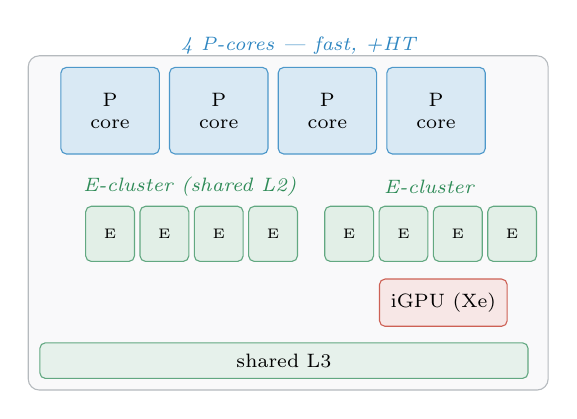
\begin{tikzpicture}[scale=0.92]
        % P cores
        \foreach \i/\x in {0/0,1/1.5,2/3.0,3/4.5}{
          \node[pcore,minimum width=1.25cm,minimum height=1.1cm] (p\i) at (\x,3.0){P\\core};}
        \node[lbl,text=oshSky] at (2.6,3.9){4 P-cores — fast, +HT};
        % E cores: two clusters of 4
        \foreach \i/\x in {0/0,1/0.75,2/1.5,3/2.25}{
          \node[ecore,minimum width=0.62cm,minimum height=0.7cm] (ea\i) at (\x,1.3){E};}
        \foreach \i/\x in {0/3.3,1/4.05,2/4.8,3/5.55}{
          \node[ecore,minimum width=0.62cm,minimum height=0.7cm] (eb\i) at (\x,1.3){E};}
        \node[lbl,text=oshGreen] at (1.1,1.95){E-cluster (shared L2)};
        \node[lbl,text=oshGreen] at (4.4,1.95){E-cluster};
        % iGPU (its own row, right side)
        \node[hot,minimum width=1.6cm,minimum height=0.6cm] (ig) at (4.6,0.35){iGPU (Xe)};
        % shared L3 bar spans the whole die, below everything
        \node[shared,minimum width=6.2cm,minimum height=0.45cm] (l3) at (2.4,-0.45){shared L3};
        \begin{scope}[on background layer]
          \node[fit=(p0)(p3)(ea0)(eb3)(l3),rounded corners,draw=oshGrey!50,
                fill=oshGrey!4,inner sep=4pt]{};
        \end{scope}
      \end{tikzpicture}\\[1mm]
      \footnotesize\color{oshGrey}
      One die, three compute classes: P-cores, E-cores, iGPU.
    \end{column}
  \end{columns}
\end{frame}

%------------------------------------------------------------------------------
\begin{frame}{The laptop is a microcosm of a hybrid node}
  \centering
  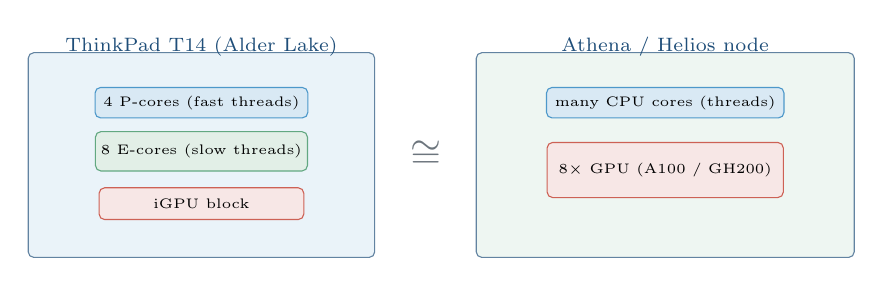
\begin{tikzpicture}[scale=0.95]
    % laptop side
    \node[box,fill=oshSky!10,minimum width=4.4cm,minimum height=2.6cm] (lap) at (0,0){};
    \node[ann] at (0,1.45){ThinkPad T14 (Alder Lake)};
    \node[pcore,minimum width=2.6cm,font=\tiny] at (0,0.7){4 P-cores (fast threads)};
    \node[ecore,minimum width=2.6cm,minimum height=0.5cm,font=\tiny] at (0,0.05){8 E-cores (slow threads)};
    \node[hot,minimum width=2.6cm,font=\tiny] at (0,-0.65){iGPU block};

    \node[font=\Large,oshGrey] at (3.0,0){$\cong$};

    % node side
    \node[box,fill=oshGreen!8,minimum width=4.8cm,minimum height=2.6cm] (nd) at (6.2,0){};
    \node[ann] at (6.2,1.45){Athena / Helios node};
    \node[pcore,minimum width=3.0cm,font=\tiny] at (6.2,0.7){many CPU cores (threads)};
    \node[hot,minimum width=3.0cm,minimum height=0.7cm,font=\tiny] at (6.2,-0.2){8$\times$ GPU (A100 / GH200)};
  \end{tikzpicture}
  \vspace{3mm}
  \begin{itemize}\small
    \item Both are \textbf{heterogeneous}: compute units of \emph{different
          speed and kind} must cooperate on one job.
    \item Whatever balances P-cores vs E-cores vs iGPU on the laptop is the
          \emph{same} mechanism that balances CPU vs GPU on a node.
    \item $\Rightarrow$ a \$300 laptop is a free, local testbed for the hardest
          part of the parallel design.
  \end{itemize}
\end{frame}

%------------------------------------------------------------------------------
\begin{frame}{Consequence (a): equal work per thread is \emph{wrong}}
  \begin{columns}[T]
    \begin{column}{0.46\textwidth}
      \small
      Split \code{nstat} into \textbf{equal} ranges (the naïve
      \code{nstat/nworkers}) and the fast cores finish early, then sit
      \textbf{idle} while the slow cores grind.
      \medskip

      On 4P+8E that idle gap is large — you can leave \textbf{30--40\,\%} of the
      machine on the floor.
      \medskip

      Static equal partitioning silently assumes \emph{homogeneous} cores.
      Alder Lake breaks that assumption on a cheap laptop — and so does every
      CPU+GPU node.
      \medskip

      \footnotesize\color{oshBlue}
      This is precisely the earlier point: ``run-by-time, or not-the-same-number
      of-primaries per thread.''
    \end{column}
    \begin{column}{0.54\textwidth}
      \centering
      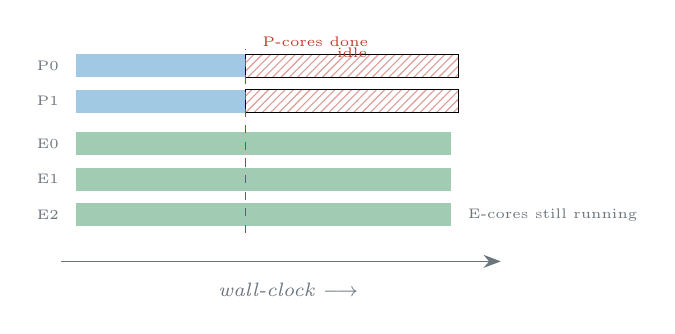
\begin{tikzpicture}[scale=0.9]
        \draw[->,oshGrey](-0.2,0)--(6.0,0);
        \node[lbl] at (3.0,-0.4){wall-clock $\longrightarrow$};
        % P-core bars (short) then idle hatch
        \foreach \i/\y in {0/2.6,1/2.1}{
          \fill[oshSky!45] (0,\y) rectangle (2.4,\y+0.32);
          \draw[pattern=north east lines,pattern color=oshRed!50]
                (2.4,\y) rectangle (5.4,\y+0.32);
          \node[lbl,font=\tiny,anchor=east] at (-0.1,\y+0.16){P\i};}
        % E-core bars (long)
        \foreach \i/\y in {0/1.5,1/1.0,2/0.5}{
          \fill[oshGreen!45] (0,\y) rectangle (5.3,\y+0.32);
          \node[lbl,font=\tiny,anchor=east] at (-0.1,\y+0.16){E\i};}
        \draw[oshRed,dashed](2.4,0.4)--(2.4,3.0);
        \node[lbl,text=oshRed,font=\tiny,anchor=west] at (2.5,3.1){P-cores done};
        \node[lbl,text=oshRed,font=\tiny] at (3.9,2.95){idle};
        \node[lbl,font=\tiny,anchor=west] at (5.4,0.66){E-cores still running};
      \end{tikzpicture}
    \end{column}
  \end{columns}
\end{frame}

%------------------------------------------------------------------------------
\begin{frame}{Fix 1 — dynamic work distribution (pull, don't pre-assign)}
  \begin{columns}[T]
    \begin{column}{0.5\textwidth}
      \small
      Don't hand each worker a fixed range. Keep one \textbf{atomic ``next
      history'' counter}; every worker \code{fetch\_add}s the next chunk when it
      finishes its current one.
      \begin{itemize}\scriptsize\itemsep2pt
        \item Fast cores naturally pull \emph{more} chunks; slow cores fewer.
        \item Self-balancing across P / E / (and a GPU block that grabs big chunks).
        \item OpenMP: one keyword — \code{schedule(dynamic, chunk)} instead of
              \code{static}.
        \item Chunked (not per-history) to keep the atomic cheap; chunk size
              trades balance vs.\ contention.
      \end{itemize}
      \footnotesize\color{oshGrey}
      The history range in \code{osh\_worker\_context} becomes a \emph{moving}
      \code{[lo,lo+chunk)} the worker refills, instead of a fixed slice.
    \end{column}
    \begin{column}{0.5\textwidth}
      \centering
      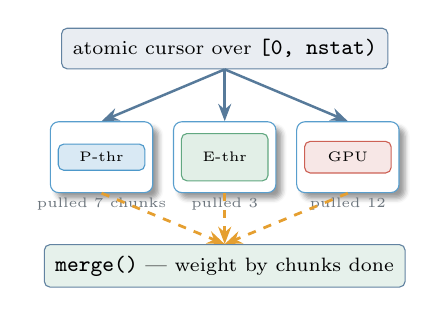
\begin{tikzpicture}[scale=0.92]
        \node[box,fill=oshBlue!10,minimum width=3.6cm] (q) at (0,3.0)
          {atomic cursor over \code{[0, nstat)}};
        \foreach \i/\x in {0/-1.7,1/0,2/1.7}{
          \node[worker,minimum width=1.3cm,minimum height=0.9cm,font=\tiny] (w\i) at (\x,1.5){};}
        \node[pcore,minimum width=1.1cm,font=\tiny] at (-1.7,1.5){P-thr};
        \node[ecore,minimum width=1.1cm,minimum height=0.6cm] at (0,1.5){E-thr};
        \node[hot,minimum width=1.1cm,font=\tiny] at (1.7,1.5){GPU};
        \foreach \i in {0,1,2}{\draw[flow](q.south)--(w\i.north);}
        % chunk tallies
        \node[lbl,font=\tiny] at (-1.7,0.85){pulled 7 chunks};
        \node[lbl,font=\tiny] at (0,0.85){pulled 3};
        \node[lbl,font=\tiny] at (1.7,0.85){pulled 12};
        \node[box,fill=oshGreen!12,minimum width=2.6cm] (m) at (0,0.0){\code{merge()} — weight by chunks done};
        \foreach \i in {0,1,2}{\draw[reduce](w\i.south)--(m.north);}
      \end{tikzpicture}
    \end{column}
  \end{columns}
\end{frame}

%------------------------------------------------------------------------------
\begin{frame}{Fix 2 — run-by-wall-time $\Rightarrow$ unequal batches (\#170)}
  \begin{columns}[T]
    \begin{column}{0.52\textwidth}
      \small
      Give every worker the \emph{same time budget} (\code{--max-time}); each
      contributes \emph{however many} histories it managed.
      \begin{itemize}\scriptsize\itemsep2pt
        \item A P-core worker finishes more primaries than an E-core worker in
              the same wall-clock window.
        \item No worker ever waits — the slow ones simply do less.
        \item Each worker is an \textbf{unequal-size batch}; total
              \code{nstat} = sum of what completed.
      \end{itemize}
      Per-history RNG makes early stop \textbf{unbiased}: the completed
      histories are a valid random subset, never ``the easy ones''.
      \medskip

      \footnotesize\color{oshGrey}
      Same primitive as a periodic dump (\#170) — and the granularity the
      variance work (\#169) already assumes.
    \end{column}
    \begin{column}{0.48\textwidth}
      \centering
      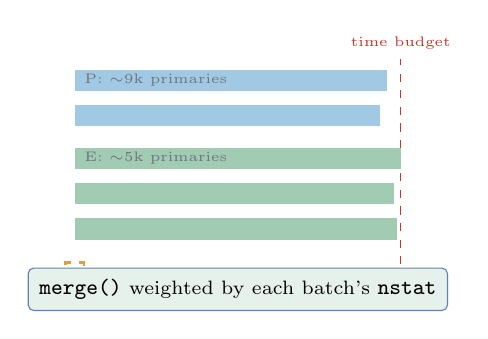
\begin{tikzpicture}[scale=0.9]
        \draw[oshRed,dashed](4.6,0.1)--(4.6,3.0);
        \node[lbl,text=oshRed,font=\tiny,anchor=south] at (4.6,3.0){time budget};
        \foreach \i/\y/\w/\c in {0/2.55/4.4/oshSky!45, 1/2.05/4.3/oshSky!45,
                                 2/1.45/4.6/oshGreen!45, 3/0.95/4.5/oshGreen!45,
                                 4/0.45/4.55/oshGreen!45}{
          \fill[\c] (0,\y) rectangle (\w,\y+0.3);}
        \node[lbl,font=\tiny,anchor=west] at (0,2.7){P: $\sim$9k primaries};
        \node[lbl,font=\tiny,anchor=west] at (0,1.6){E: $\sim$5k primaries};
        \node[reduce] at (0,0) {};
        \node[box,fill=oshGreen!12,minimum width=3.0cm] at (2.3,-0.25)
          {\code{merge()} weighted by each batch's \code{nstat}};
      \end{tikzpicture}
    \end{column}
  \end{columns}
\end{frame}

%------------------------------------------------------------------------------
\begin{frame}{Why the existing design already supports unequal work}
  \centering
  \small Nothing new is needed in the engine — only \emph{how} ranges are sized and
  the merge is weighted.
  \vspace{2mm}

  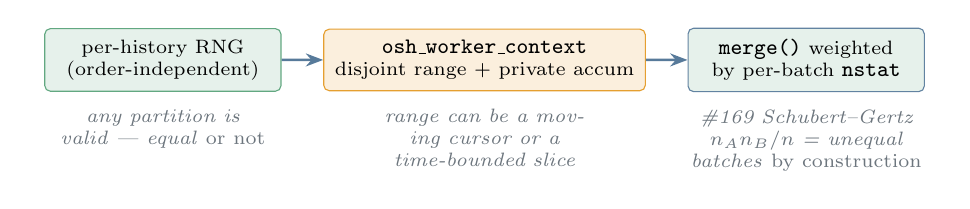
\begin{tikzpicture}[scale=0.95]
    \node[shared,minimum width=3.0cm] (a) at (0,2.4)
      {per-history RNG\\(order-independent)};
    \node[private,minimum width=3.0cm] (b) at (4.3,2.4)
      {\code{osh\_worker\_context}\\disjoint range + private accum};
    \node[box,fill=oshGreen!12,minimum width=3.0cm] (c) at (8.6,2.4)
      {\code{merge()} weighted\\by per-batch \code{nstat}};
    \draw[flow](a)--(b); \draw[flow](b)--(c);
    \node[lbl,below=1mm of a,text width=3.2cm,align=center]
      {any partition is valid — equal \emph{or not}};
    \node[lbl,below=1mm of b,text width=3.2cm,align=center]
      {range can be a moving cursor or a time-bounded slice};
    \node[lbl,below=1mm of c,text width=3.2cm,align=center]
      {\#169 Schubert--Gertz $n_A n_B/n$ = unequal batches \emph{by construction}};
  \end{tikzpicture}
  \vspace{3mm}
  \begin{itemize}\scriptsize
    \item The \textbf{only} requirement: the merge must \textbf{weight by each
          worker's primary count} (the \code{.bdo} NORM/AVER rules already do
          exactly this).
    \item So Niels' hybrid-CPU observation is independent confirmation that the
          \emph{unequal-batch / run-by-time} path was the right call.
  \end{itemize}
\end{frame}

%------------------------------------------------------------------------------
\begin{frame}{Consequence (b): the usable SIMD width drops to AVX2}
  \begin{columns}[T]
    \begin{column}{0.54\textwidth}
      \small
      The E-cores (Gracemont) don't implement \textbf{AVX-512}. A thread can
      migrate between core types, so the two types \emph{must} expose the same
      instruction set $\Rightarrow$ Intel \textbf{fused AVX-512 off} on consumer
      Alder Lake.
      \medskip

      \textbf{Rule:} a hybrid CPU's usable ISA is the \textbf{lowest common
      denominator} across its core types.
      \begin{itemize}\scriptsize\itemsep2pt
        \item T14 (Alder Lake): rely on \textbf{AVX2} (256-bit, 4 doubles).
        \item Ares (Cascade-Lake) / Helios (Genoa): homogeneous
              \textbf{AVX-512} (8 doubles).
        \item Athena (Rome EPYC): AVX2 only — homogeneous, but narrower.
      \end{itemize}
      $\Rightarrow$ \textbf{detect width at runtime} and dispatch, rather than
      hard-assume AVX-512 at compile time. One binary, optimal on laptop and
      cluster.
    \end{column}
    \begin{column}{0.46\textwidth}
      \centering
      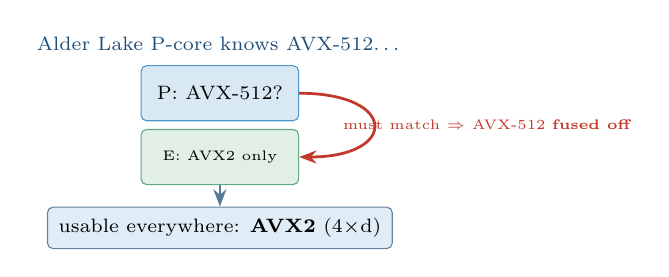
\begin{tikzpicture}[scale=0.9]
        \node[ann] at (0,3.0){Alder Lake P-core knows AVX-512\dots};
        \node[pcore,minimum width=2.0cm,minimum height=0.7cm] (p) at (0,2.3){P: AVX-512?};
        \node[ecore,minimum width=2.0cm,minimum height=0.7cm] (e) at (0,1.4){E: AVX2 only};
        \draw[->,oshRed,line width=1pt] (p.east) .. controls +(1.4,0) and +(1.4,0) .. (e.east);
        \node[lbl,text=oshRed,font=\tiny,anchor=west] at (1.6,1.85){must match $\Rightarrow$ AVX-512 \textbf{fused off}};
        \node[box,fill=oshSky!15,minimum width=3.4cm] (use) at (0,0.4)
          {usable everywhere: \textbf{AVX2} (4$\times$d)};
        \draw[flow](e.south)--(use.north);
      \end{tikzpicture}
    \end{column}
  \end{columns}
\end{frame}

%------------------------------------------------------------------------------
\begin{frame}{Hybrid in the HPC sense — the strategies compose}
  \centering
  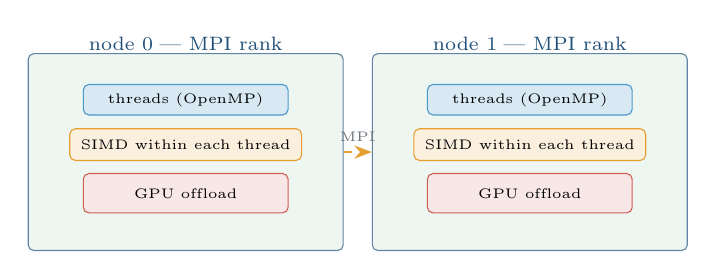
\begin{tikzpicture}[scale=0.95]
    % nodes
    \foreach \r/\x in {0/0,1/4.6}{
      \node[box,fill=oshGreen!8,minimum width=4.0cm,minimum height=2.5cm] (n\r) at (\x,0){};
      \node[ann] at (\x,1.45){node \r \;— MPI rank};
      \node[pcore,minimum width=2.6cm,font=\tiny] at (\x,0.7){threads (OpenMP)};
      \node[private,minimum width=2.6cm,font=\tiny] at (\x,0.1){SIMD within each thread};
      \node[hot,minimum width=2.6cm,minimum height=0.5cm,font=\tiny] at (\x,-0.55){GPU offload};
    }
    \draw[reduce] (n0.east) -- node[lbl,above,font=\tiny]{MPI} (n1.west);
  \end{tikzpicture}
  \vspace{2mm}
  \begin{itemize}\small
    \item \textbf{MPI $\times$ OpenMP:} ranks across nodes, threads within —
          big read-only tables load \emph{once per node}, not once per rank
          (matters as cross-sections grow). $=$ the \textbf{A $\times$ B} composition.
    \item \textbf{CPU $+$ GPU:} cores \emph{and} GPU(s) pull from the same job,
          merged at the end $=$ \textbf{A/B $\times$ D}.
    \item Each level reuses the \emph{same} contract: range $\to$
          \code{run\_history\_range} $\to$ private accumulator $\to$
          \code{merge}.
  \end{itemize}
\end{frame}

%------------------------------------------------------------------------------
\begin{frame}{The unifying idea: a ``compute unit'' abstraction}
  \begin{columns}[T]
    \begin{column}{0.46\textwidth}
      \small
      Make a \textbf{worker} polymorphic. A P-core thread, an E-core thread, an
      MPI rank and a GPU block all present the \emph{same} four-step contract:
      \medskip

      \begin{enumerate}\scriptsize\itemsep2pt
        \item take a history range (fixed, cursor-pulled, or time-bounded),
        \item \code{run\_history\_range()} over it,
        \item deposit into a \textbf{private} accumulator,
        \item \code{merge()} into the master, weighted by primaries done.
      \end{enumerate}
      \medskip
      Heterogeneity then lives in \emph{one} place — how big a bite each unit
      takes — not smeared through transport or scoring. That is what makes
      ``hybrid'' cheap rather than a rewrite.
    \end{column}
    \begin{column}{0.54\textwidth}
      \centering
      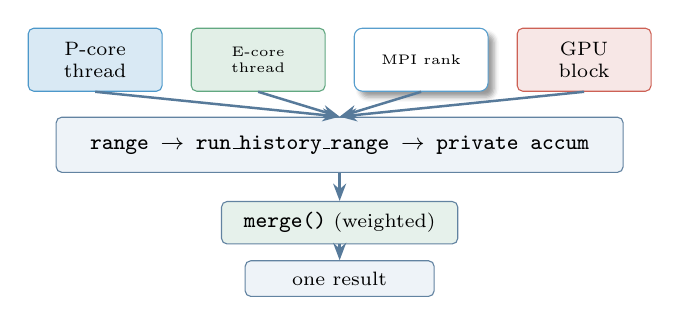
\begin{tikzpicture}[scale=0.9]
        \node[pcore,minimum width=1.7cm,minimum height=0.8cm] (p) at (0,3.0){P-core\\thread};
        \node[ecore,minimum width=1.7cm,minimum height=0.8cm] (e) at (2.3,3.0){E-core\\thread};
        \node[worker,minimum width=1.7cm,minimum height=0.8cm,font=\tiny] (r) at (4.6,3.0){MPI rank};
        \node[hot,minimum width=1.7cm,minimum height=0.8cm] (g) at (6.9,3.0){GPU\\block};
        \node[box,fill=oshLight,minimum width=7.2cm,minimum height=0.7cm] (api) at (3.45,1.8)
          {\code{range $\to$ run\_history\_range $\to$ private accum}};
        \foreach \n in {p,e,r,g}{\draw[flow](\n.south)--(api.north);}
        \node[box,fill=oshGreen!12,minimum width=3.0cm] (m) at (3.45,0.7){\code{merge()} (weighted)};
        \draw[flow](api.south)--(m.north);
        \node[box,minimum width=2.4cm,below=2mm of m](out){one result};
        \draw[flow](m)--(out);
      \end{tikzpicture}
    \end{column}
  \end{columns}
\end{frame}

%------------------------------------------------------------------------------
\begin{frame}{Discussion points this opens (for Thursday)}
  \small
  \begin{enumerate}\itemsep3pt
    \item \textbf{Scheduling policy.} Dynamic chunked pull (atomic counter /
          \code{schedule(dynamic)}) vs.\ run-by-wall-time — both give unequal
          batches. Want both, with \code{--threads} defaulting to dynamic?
    \item \textbf{Weighted merge from day one.} Verify the merge contract
          (\#169) combines unequal \code{n} correctly, so a P-core batch and an
          E-core batch fold without bias.
    \item \textbf{Runtime ISA dispatch.} Detect AVX2 vs AVX-512 (and core type)
          at runtime, not compile time — one binary optimal on the hybrid
          laptop \emph{and} a homogeneous AVX-512 node.
    \item \textbf{Affinity / oversubscription.} On P+E, bind 1 thread per
          logical CPU (incl.\ P-core HT) or 1 per physical core? Needs
          measuring; differs from a plain Xeon.
    \item \textbf{Unified compute-unit abstraction.} Adopt the polymorphic
          worker (P / E / rank / GPU block) so heterogeneity stays in one
          place.
  \end{enumerate}
  \vspace{2mm}
  \footnotesize\color{oshGrey}
  The T14 is a ready-made test rig for points 1, 2 and 4 — measurable today on
  hardware Niels already owns.
\end{frame}

\begin{frame}[plain]
  \centering
  \vfill
  {\Large\color{oshBlue}\textbf{End of backup}}\\[2mm]
  \small\color{oshGrey}
  Heterogeneous hardware forces unequal work $\Rightarrow$ dynamic / time-based
  distribution + weighted merge.\\
  The existing \#162 seams (worker context $\cdot$ private accumulator $\cdot$
  merge) already carry it; ``hybrid'' is a policy on top, not a rewrite.
  \vfill
\end{frame}

\end{document}
